\documentclass[tikz,border=4pt]{standalone}
\usepackage{lmodern}
\usetikzlibrary{shadings}
% The graph G_3 of the paper, in four layers. Shaded vertices form the minimal 3-star-forming set S;
% white vertices are p, q_1, q_2. Red edges are the three stars K_{1,3} that certify p, q_1, q_2.
\begin{document}
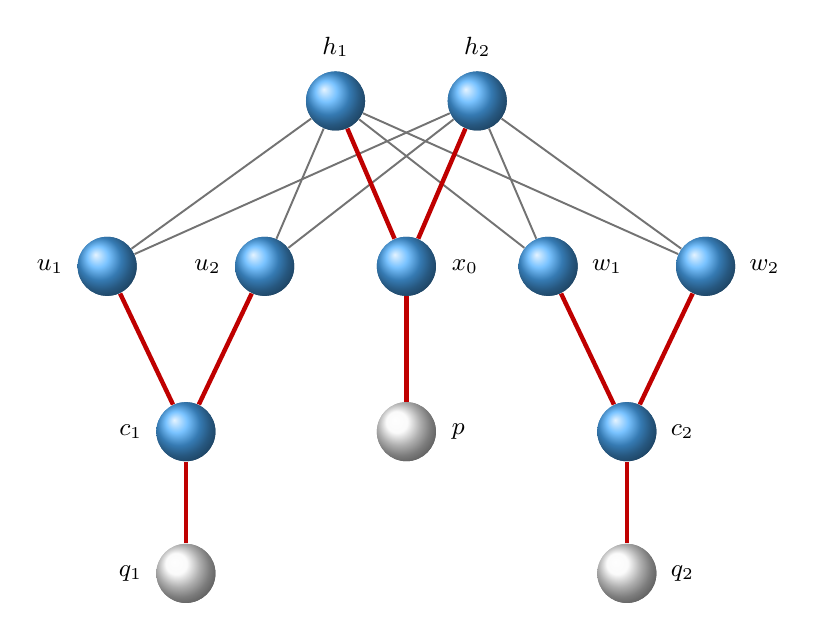
\begin{tikzpicture}[
    inS/.style={circle, minimum size=7.5mm, inner sep=0pt, shading=ball, ball color=blue!45!cyan!70},
    outS/.style={circle, minimum size=7.5mm, inner sep=0pt, shading=ball, ball color=white!95!gray},
    lab/.style={font=\small},
    e/.style={line width=0.7pt, black!55},
    cert/.style={line width=1.6pt, red!75!black},
  ]
  % layer 1: hubs
  \node[inS] (h1) at (2.35, 2.1) {};
  \node[inS] (h2) at (4.15, 2.1) {};
  % layer 2: X = X_1 + {x_0} + X_2
  \node[inS] (u1) at (-0.55, 0) {};
  \node[inS] (u2) at (1.45, 0) {};
  \node[inS] (x0) at (3.25, 0) {};
  \node[inS] (w1) at (5.05, 0) {};
  \node[inS] (w2) at (7.05, 0) {};
  % layer 3
  \node[inS] (c1) at (0.45, -2.1) {};
  \node[outS] (p) at (3.25, -2.1) {};
  \node[inS] (c2) at (6.05, -2.1) {};
  % layer 4
  \node[outS] (q1) at (0.45, -3.9) {};
  \node[outS] (q2) at (6.05, -3.9) {};
  % edges
  \foreach \h in {h1, h2} \foreach \x in {u1, u2, w1, w2} \draw[e] (\h) -- (\x);
  \draw[cert] (h1) -- (x0); \draw[cert] (h2) -- (x0); \draw[cert] (x0) -- (p);
  \draw[cert] (c1) -- (u1); \draw[cert] (c1) -- (u2); \draw[cert] (c1) -- (q1);
  \draw[cert] (c2) -- (w1); \draw[cert] (c2) -- (w2); \draw[cert] (c2) -- (q2);
  % redraw the vertices on top of the edges
  \foreach \v/\s in {h1/inS, h2/inS, u1/inS, u2/inS, x0/inS, w1/inS, w2/inS, c1/inS, c2/inS,
                     p/outS, q1/outS, q2/outS} \node[\s] at (\v) {};
  % labels
  \node[lab, above=1.5pt] at (h1.north) {$h_1$};
  \node[lab, above=1.5pt] at (h2.north) {$h_2$};
  \node[lab, left=1.5pt] at (u1.west) {$u_1$};
  \node[lab, left=1.5pt] at (u2.west) {$u_2$};
  \node[lab, right=2pt] at (x0.east) {$x_0$};
  \node[lab, right=1.5pt] at (w1.east) {$w_1$};
  \node[lab, right=1.5pt] at (w2.east) {$w_2$};
  \node[lab, left=1.5pt] at (c1.west) {$c_1$};
  \node[lab, right=2pt] at (p.east) {$p$};
  \node[lab, right=1.5pt] at (c2.east) {$c_2$};
  \node[lab, left=1.5pt] at (q1.west) {$q_1$};
  \node[lab, right=1.5pt] at (q2.east) {$q_2$};
\end{tikzpicture}
\end{document}
